%SDES_Project_1
%Vinod Kumar Metla
%130010048
\documentclass[12pt, a4paper]{report}

%for matrix
\usepackage{amsmath}

%for placing the figures at the correct place
\usepackage{placeins}

%for Graphics
\usepackage{graphicx}
\graphicspath{{images/}}

%for including specific amount of space
\newcommand\tab[1][1cm]{\hspace*{#1}}

\usepackage[affil-it]{authblk}
\usepackage{etoolbox}
\usepackage{lmodern}
\usepackage{titlesec}
\usepackage{float}
\usepackage{amsfonts}
\usepackage[pdfpagelabels]{hyperref}

\makeatletter
\patchcmd{\@maketitle}{\LARGE \@title}{\fontsize{20}{19.2}\selectfont\@title}{}{}
\makeatother

\renewcommand\Authfont{\fontsize{16}{14.4}\selectfont}
\renewcommand\Affilfont{\fontsize{12}{10.8}\itshape}

%for hyperlinks
\usepackage[english]{babel}

%for header
\usepackage[utf8]{inputenc}
\usepackage{fancyhdr}
 
\usepackage{hyperref}
\hypersetup{
    colorlinks=true,
    linkcolor=blue,
    filecolor=magenta,      
    urlcolor=cyan,
} 
\urlstyle{same}

\title{\textbf{LC Tank with Resistance}}
\author{Vinod Kumar Metla}
\affil{Roll No. : 130010048}

\begin{document}
\maketitle
\newpage

\begin{abstract}
 The problem is to simulate the behaviour of a LC tank with a resistance applied across a voltage in series with given initial conditions of the charge in the capacitor and current in the inductor.
\end{abstract}

\begin{itemize}
\item Public git repo with open source code is available on \url{https://github.com/vinodm24/sdes_project_1}
\item Ipython 2.3.0 is used to run the IPython notebook. So the version 2.3.0 or higher is preferrable to run the notebook.
\item numpy version 1.8.2 is used. So numpy version 1.8.2 or higher is preffered to run the code.
\item matplotlib version 1.4.2 is used. So matplotlib version 1.4.2 or higher is preffered to run the code. 
\end{itemize}

\section*{Governing Equation for the problem}
The governing equation for this electrical problem is 
\begin{equation}
 \frac{d^2Q}{dt^2} + \frac{R}{L}\frac{dQ}{dt} + \frac{Q}{LC} = \frac{V}{C}
\end{equation}

where $Q$ is the charge in the capacitor varying with time, R is the resistance in the circuit, L is inductance of the inductor,C is the capacitance of the capacitor and V is the voltage of the source voltage under the initial conditions of $Q(0^+) = Q_0$ the initial charge in the capacitor and $\frac{dQ}{dt}(0^+) = i_0$, where initial inductor current is $i_0$. \\

Solving this analytically for two cases of $\Delta = 0$ and $\Delta \ne 0$ where $\Delta = \frac{R^2}{L^2} - \frac{4}{LC}$ \\
\subsection*{$\Delta = 0$ :}
The solution when $\Delta = 0$ under the given initial conditions is:
\begin{equation}
 Q(t) = CV + e^\frac{-2Lt}{R}(C_1t + C_2)
\end{equation}
where $C_1 = i_0+\frac{R}{2L}(Q_0-CV) , C_2 = (Q_0 - CV)$
\subsection*{$\Delta \ne 0$ :}
The solution when $\Delta \ne 0$ under the given initial conditions is:
\begin{equation}
 Q(t) = CV + A_1e^{s_1t} + A_2e^{s_2t}
\end{equation}
where $s_1 = \frac{-R}{2L} + \frac{\sqrt{\Delta}}{2} , s_2 = \frac{-R}{2L} - \frac{\sqrt{\Delta}}{2}$ \\
$A_1 = \frac{i_0 - (Q_0 - CV)s_2}{s_1 - s_2} , A_2 = \frac{i_0 - (Q_0 - CV)s_1}{s_2 - s_1}$ \\
\\

The results were plotted showing the voltage across all the elements of the circuit varying with time for three cases of damping.\\

\textbf{Under Damped case}
\begin{figure}[H]
  \centering
  \fbox{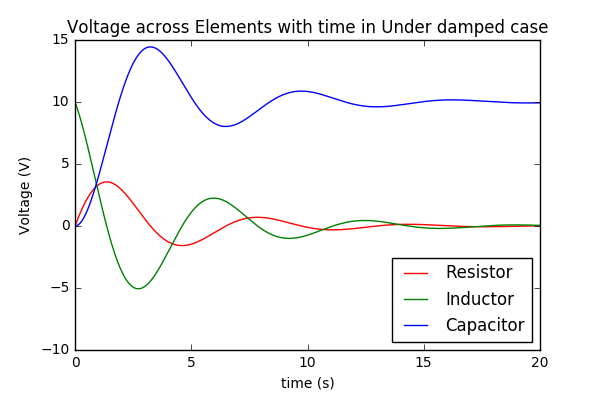
\includegraphics[scale=0.7]{voltage_across_elements_in_underdamped_case}}
  \caption[Voltage vs time]    
  {\textit{Voltage vs time}
  \label{Fig:1}
  \footnotemark.}
\end{figure}
\pagebreak
\textbf{Critically Damped case}
\begin{figure}[H]
  \centering
  \fbox{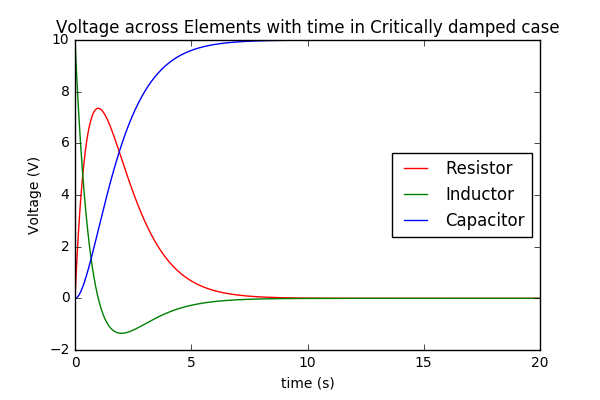
\includegraphics[scale=0.7]{voltage_across_elements_in_criticallydamped_case}}
  \caption[Voltage vs time]    
  {\textit{Voltage vs time}
  \label{Fig:2}
  \footnotemark.}
\end{figure}
\textbf{Over Damped case}
\begin{figure}[H]
  \centering
  \fbox{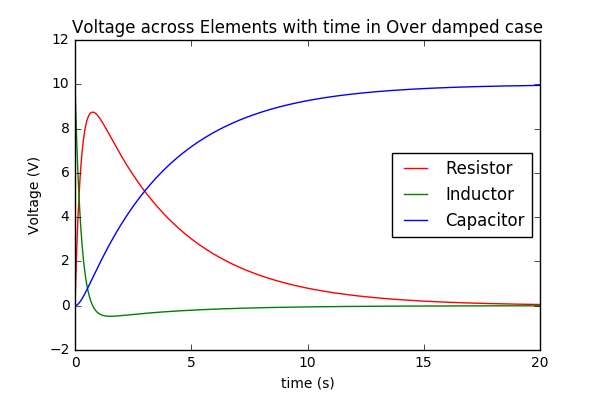
\includegraphics[scale=0.7]{voltage_across_elements_in_overdamped_case}}
  \caption[Voltage vs time]    
  {\textit{Voltage vs time}
  \label{Fig:2}
  \footnotemark.}
\end{figure}
\end{document}